\subsection{Descripción del método TAMA}
\label{sec:ant_tama}

En \cite{KOU2008} se introdujo un método novedoso para el análisis del \entrainment acústico-prosódico. Esta técnica consiste en armar dos series de tiempo para cada uno de los interlocutores y luego utilizar herramientas de análisis bivariado sobre las series construídas. 

Para construir la serie de tiempo de cada hablante debemos, en primer lugar, dividir el diálogo en ventanas solapadas de igual tamaño. A la diferencia entre ventana y ventana llamaremos \emph{frame step}, y al tamaño de ventana \emph{frame length}. Consideraremos sólo los segmentos de habla que tengan intersección con la ventana dentro de cada ventana. En la Figura \ref{tama} se ilustra el proceso: las líneas punteadas marcan los límites de la ventana, los intervalos coloreados en negro los segmentos de habla, y en gris los segmentos no considerados.

\begin{figure}[t]
\centering
  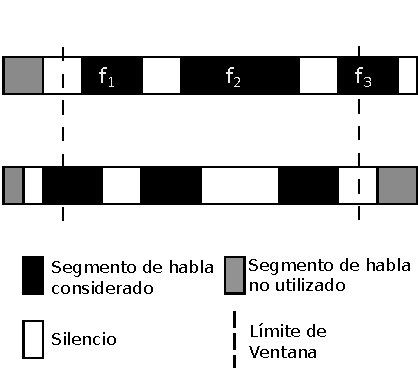
\includegraphics[scale=0.85]{images/tama_improved.pdf}
\caption{Gráfico de la separación del diálogo en ventanas. Fuente \cite{KOU2008.2}}
\label{tama}
\end{figure}

Luego se calculan los valores de la serie de tiempo para cada hablante y cada variable acustico-prosódica mediante la siguiente fórmula:

\begin{equation}
    \mu = \sum\limits_{i=1}^N f_i d_i^\prime \label{eq:tama_mean}\\
\end{equation}

\noindent donde $i$ itera sobre las elocuciones dentro del \emph{frame}, $d_i^\prime$ es la duración relativa del segmento (respecto del tiempo total hablado en toda la ventana) y $f_i$ es el valor de la \emph{variable acústico-prosódica} que estamos midiendo.

Como se ve en la ecuación \ref{eq:tama_mean}, el valor que calculamos es una media ponderada del valor de la variable por la duración de las elocuciones. Así, por ejemplo, al calcular una serie de tiempo sobre la intensidad, la contribución de interjecciones (\emph{ah!} por ejemplo), que suelen tener altos valores, estará atenuada por sus breves duraciones.

\newcommand{\squarederr}[1]{
    \sum\limits_{t=1}^n \varnorm{#1}^2
}

\newcommand{\crosscorr}[2]{
  \frac{\sum\limits_{t=|k|+1}^n \varnorm{#1} (#2_{t-k} - \mu_{#2})}{
    \sqrt{\squarederr{#1} \squarederr{#2}}
  } \\
}

\newcommand{\corrdenom}{\sqrt{\squarederr{A}\squarederr{B}}}


Una vez obtenidas las series de tiempo respectivas, una posible medida del \entrainment se puede obtener midiendo cuánto influye una serie sobre otra, considerándolas a ambas como parte de un sistema donde ambas interactúan. Este \entrainment, entonces, sería direccional: queremos medir cuánto influye el interlocutor $A$ sobre el interlocutor $B$ y viceversa. Puede darse el caso en que ambos tengan fuerte interacción, en tal caso hablamos de \emph{feedback}.

Para medir cuánto se mimetizan las dos series, se usa la función de correlación cruzada (f.c.c) \cite{CHATFIELD}, que mide cuánto se parecen la serie $X$ e $Y$ aplicando un desplazamiento $k$, lo cual nos arroja como resultado un valor entre $-1$ y $1$ (similar al coeficiente de correlación de la estadística clásica). Podemos aproximar la c.c.f. mediante la fórmula de la correlación cruzada muestral.

\begin{equation}
  \label{cross_correlation_definition}
  r_{AB}(k) =
  \left\{
    \begin{array}{ll}
      \frac{\sum\limits_{t=k+1}^n \varnorm{A} (B_{t-k} - \mu_{B})}{\corrdenom} \\ & \mbox{si } k \geq 0 \\
      \frac{\sum\limits_{t=-k+1}^n \varnorm{B} (A_{t+k} - \mu_{A})}{\corrdenom} \\  & \mbox{si } k < 0
    \end{array}
  \right.
\end{equation}

Podemos ver que, si $k \geq 0$, lo que hacemos es, a grandes rasgos, calcular la correlación de Pearson entre $A$ y $B$, pero tomando los $n-k$ últimos valores de $A$ y los $n-k$ primeros de $B$. Si $k < 0$, lo hacemos entre $A$ y $B$, pero desplazando en sentidos inversos. Viéndolo de otra forma, si $k \geq 0$, estamos midiendo cuánto influye $B$ sobre $A$ contemplando un desplazamiento de $k$ puntos; si $k \leq 0$ medimos la influencia de $A$ sobre $B$ a misma distancia. La utilización de estos desplazamientos está explicada en \cite{gravano2015backward}, donde se menciona que la influencia de los hablantes no es necesariamente inmediata sino que puede tener algunos segundos de demora para tomar lugar. 

Para cada conversación, se estima entonces el correlograma cruzado, considerando desplazamientos tanto positivos como negativos. Hecho esto, en el estudio \cite{KOU2008.2} sólo analizan la significancia de los resultados de la correlación cruzada, enumerando aquellos lags en los cuales esto ocurrió.

\begin{figure}[b]
\centering
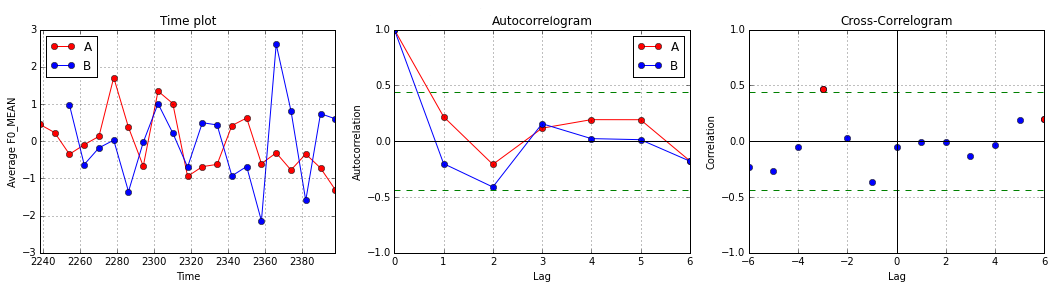
\includegraphics[width=\textwidth]{images/time_plot_with_cross_correlation.png}
\caption{Time-plot producido por TAMA, junto a su autocorrelación y correlación cruzada}
\end{figure}


\subsection{TAMA sobre Columbia Games}
\label{sec:tama_modifications}

En \cite{KOU2008.2} se discute la disyuntiva de elegir un tamaño de ventana y step para el método: ventanas demasiado chicas pueden causar que no hayan segmentos de habla en ellas, mientras que un tamaño de ventana demasiado grande suavizaría en exceso la serie de tiempo. También se mencionan dos posibles soluciones para el problema de los puntos faltantes: interpolar\cite{DEL2013} o repetir el punto anterior de la serie. Estos enfoques, sin embargo, pueden dar lugar a valores de \entrainment artificialmente altos  por la construcción misma de la serie, ya que nos generaría puntos correlacionados fuertemente entre sí en cada una de las series de los hablantes. Por otro lado, descartar aquellas conversaciones que tengan puntos faltantes puede ser demasiado restrictivo y eliminar de nuestro corpus una gran cantidad de datos valiosos. Teniendo estas cosas en mente, decidimos aceptar series de tiempo con datos faltantes, que pueden ser producto de ventanas sin segmentos de habla o con algunos demasiado pequeños que imposibiliten la medición de las variables \ap.

A su vez, se modificó el tamaño de la ventana para ajustarlo a nuestro corpus. En vez del step de 10'' y tamaño de 20'', optamos por 8 y 16 segundos respectivamente luego de efectuar un análisis con el fin de encontrar un balance entre el tamaño de la ventana y la cantidad de indefiniciones. Considerando estos parámetros, se procedió a calcular las dos series de tiempo para cada conversación y cada variable acústico-prosódica. De estas tareas, sólo nos quedamos con aquellas que tengan al menos 5 puntos definidos para cada serie, de manera que tenga sentido poder calcular la correlación cruzada más adelante. Con esto, no sólo nos interesa la duración de la charla, sino cierta calidad de las series generadas.

Finalmente, definimos una primer métrica de \entrainment $\fwentrainment{AB}^{(1)}$ como el valor de $r_{AB}(k)$ con mayor valor absoluto, dado $k \leq 0$. Análogamente lo definimos para $\fwentrainment{BA}^{(1)}$, usando $k \geq 0$. Además, definimos una segunda métrica $\fwentrainment{BA}^{(2)}$, como el valor absoluto de la primera, es decir $\fwentrainment{BA}^{(2)} = |\fwentrainment{BA}^{(1)}|$. Esta segunda métrica considera de forma positiva la asincronía entre las series de tiempo, también conocido en la literatura como antimimicry o \disentrainment\cite{CHAR1999}.

Este fenómeno refiere al proceso por el cual uno de los hablantes no imita al otro sino más bien todo lo contrario, acentúa alguna diferencia. Si bien estudios de larga data como \cite{bourhis1973language} o \cite{dabbs1969similarity} lo emparentan con una connotación negativa, \cite{healey2014divergence} y \cite{levitan2015acoustic} sugieren que puede entenderse este fenómeno como una conducta de adaptación cooperativa. No sólo eso, sino que este fenómeno de mimetización complementaria podría ser incluso más prevalente que la mimetización a secas \cite{levitan2015acoustic}.
